
\documentclass[
                                          %
   12pt,                                % Schriftgroesse 12pt
   a4paper,                             % Layout fuer Din A4
   twoside,                             % Layout fuer beidseitigen Druck
   headinclude,                         % Kopfzeile wird Seiten-Layouts mit beruecksichtigt
   headsepline,                         % horizontale Linie unter Kolumnentitel
   plainheadsepline,                    % horizontale Linie auch beim plain-Style
   BCOR18mm,                            % Korrektur fuer die Bindung
   DIV14,                               % DIV-Wert fuer die Erstellung des Satzspiegels, siehe scrguide
   parskip=half,                        % Absatzabstand statt Absatzeinzug
   bibliography=totoc,                  % Literaturverz. wird ins Inhaltsverzeichnis eingetragen
   captions=tableheading,               % korrekte Abstaende bei TabellenUEBERschriften
%   openany,                            % Kapitel k�nnen auf geraden und ungeraden Seiten beginnen
   listof=totoc,                         % Abbildungs- und Tabellenverzeichnis in Inhaltsverz.
%   pointlessnumbers,                   % Kapitelnummern immer ohne Punkt
%   fleqn,                              % fleqn: Glgen links (statt mittig)
%  draft                               % Keine Bilder in der Anzeige, overfull hboxes werden angezeigt
%   chapterprefix,                      % x. Kapitel �ber Kapitel�berschrift schreiben
     ]{scrbook}[2001/07/30]             % scrbook-Version mind. 2.8j von 2001/07/30

%makeindex Studienarbeit.nlo -s nomencl.ist -o Studienarbeit.nls
\usepackage{ngerman}                    % neue Rechtschreibung
%\usepackage[english]{babel}          % falls man in Englisch schreiben will
\selectlanguage{german}
%\selectlanguage{english}               % falls man in Englisch schreiben will
\usepackage{bibgerm}                    % Dt. Bibliothek 

\usepackage[latin1]{inputenc}           % Input-Encodung: latin1 fuer Unix
\usepackage[T1]{fontenc}                % T1-kodierte Schriften, korrekte Trennmuster fuer Worte mit Umlauten
\usepackage{ae}                         % F�r PDF-Erstellung
%\usepackage[hang]{caption2}             % mehrzeilige Captions ausrichten
%\usepackage{pifont}                     % f�r Zahlen im Kreis mit \ding{202} Google: symbols-a4.ps
\usepackage{graphicx}                   % zum Einbinden von Grafiken
\usepackage{float}                      % u.a. genaue Plazierung von Gleitobjekten mit H
\usepackage{tabularx}
\usepackage{amsmath}
\usepackage{amsfonts}
\usepackage{dsfont}
\usepackage{scrhack}
%  \newshadetheorem{definition}{Definition}
%  \newshadetheorem{folgerung}{Folgerung}
%  \newshadetheorem{thm}{Theorem}
  
%\usepackage{draftwatermark}
  
%\DeclareMathOperator{\grad}{grad}

%------------------Anfang Nummerierung Anhang-----------------
 \renewcommand\appendix{\par 
   \setcounter{section}{0}% 
   \setcounter{subsection}{0}% 
   \setcounter{figure}{0}%
   \renewcommand\thesection{\Alph{section}}% 
   \renewcommand\thefigure{\Alph{section}.\arabic{figure}}
   \renewcommand\theequation{\Alph{section}.\arabic{equation}}} 
%------------------Ende Nummerierung Anhang-----------------
%\usepackage{tocbasic}
\usepackage{wrapfig}
\usepackage{longtable}
%\usepackage{subfigure}
\usepackage{subfigure}
%\usepacka{gemes=falsre
%   colorlinks,linkcolor={black},citecolor={black},urlcolor={red},
%   pdfstartview={FitV},unicode,breaklinks=false]{hyperref}
%\usepackage{natbib}
% fuer Stichwortverzeichnis
%\usepackage{makeidx}
%\makeindex
%\renewcommand{\indexname}{Stichwortverzeichnis}
                                        % falls der Index nicht "`Index"' heissen soll
%\addcontentsline{toc}{section}{Stichwortverzeichnis}
                                        % falls das Stichwortverzeichnis im Inhaltsverzeichnis auftauchen soll


%\usepackage[ansinew]{inputenc}
                                        % Input-Encodung: ansinew fuer Windows

%\usepackage[centertags]{amsmath}
                                        % AMS-Mathematik, centertags zentriert Nummer bei split
%\usepackage{latexsym}
                                        % verschiedene Symbole
%\usepackage{textcomp}
                                        % verschiedene Symbole
\usepackage{pstricks}
%\usepackage{pst-all}
%                                        % PostScript Macros
\usepackage{psfrag}
\usepackage{pst-node}
\usepackage{psfrag}

%\usepackage{pstricks-add}  								% Standard PSTricks Paket
%\usepackage{pst-3dplot}								% 3D Plots mit PSTricks 
							% zus�tzliche PSTRicks Funktionalit�t
%\usepackage{rotating}	
%%%%%%%%%%%%%%%%%%%%%%%%%%%%%%%%%%%%%%%%%%%%%%%%%%%%%%
% M A K R O S   U N D   D E F I N I T I O N E N
%%%%%%%%%%%%%%%%%%%%%%%%%%%%%%%%%%%%%%%%%%%%%%%%%%%%%%

%%%%%%%%%%%%%%%%%%%% Symbole %%%%%%%%%%%%%%%%%%%%%%%%%


%%%%%%%%%%%%%%%%%%%%%%% PSTricks %%%%%%%%%%%%%%%%%%%%%%%%%%

%% Zur�cksetzen aller ver�nderten Werte
\newcommand{\psreset}{%
\psset{unit      = 1mm,
       xunit     = 1mm,
       yunit     = 1mm,
       linewidth = 1pt,
       linestyle = solid,
       linecolor = black,
       fillstyle = solid,
       fillcolor = white,
       Beta      = 0,
       Alpha     = 0}}

% Textgr��e
\newcommand{\textscale}{1}
% Liniendicken f�r Zeichnungen
\newlength{\lwFine}   \pssetlength{\lwFine}{0.1mm} % = 0.14mm
\newlength{\lwfine}   \pssetlength{\lwfine}{0.2mm} % = 0.14mm
\newlength{\lwnormal} \pssetlength{\lwnormal}{0.3mm} % = 0.21mm
\newlength{\lwthick}  \pssetlength{\lwthick}{0.5mm}
\newlength{\lwThick}  \pssetlength{\lwThick}{0.75mm} % = 0.64mm%

% verschiedene style Definitionen
\newpsstyle{normal}{arrowsize=1pt 3,arrowlength=2,arrowinset=0, linewidth=\lwnormal}%
\newpsstyle{koordpfeil}{arrowsize=2 0,arrowlength=2.5,arrowinset=0}%
%\newpsstyle{kdpfeil}{arrowsize=1.5 0,arrowlength=1.875,arrowinset=0,linewidth=\lwfine}%
\newpsstyle{masspfeil}{linewidth=\lwfine, arrowsize=2 0,arrowlength=2.5,arrowinset=0}%
%\newpsstyle{dottedline}{linestyle=dotted,dotsep=2pt}

\newpsstyle{PSGraphDash}{plotstyle=line,linewidth=0.8pt,linestyle=dashed,dash=4pt 4pt}
\newpsstyle{PSGraphSolidDot}{plotstyle=line,linewidth=0.8pt,linestyle=solid,showpoints=true}
\newpsstyle{PSGraphDot}{plotstyle=line,linewidth=1.2pt,linestyle=dotted,dotsep=2pt}
\newpsstyle{PSGraphDashDot}{plotstyle=line,linewidth=0.8pt,linestyle=dashed,dash=4pt 2pt 0.6pt 2pt}
\newpsstyle{PSGraphSolid}{plotstyle=line,linewidth=0.8pt,linestyle=solid}
\newpsstyle{PSGraphDashDotDot}{plotstyle=line,linewidth=0.8pt,linestyle=dashed,dash=4pt 2pt 0.6pt 2pt 0.6pt 2pt}
\newpsstyle{PSGraphPoint}{plotstyle=dots,dotstyle=*,dotsize=1.5}
% Schraffuren
\newpsstyle{hatchedu}{fillstyle=hlines,hatchwidth=\lwfine}
\newpsstyle{hatchedd}{fillstyle=vlines,hatchwidth=\lwfine}

%%%%%%%%%%%%%%%%%%%%%%%%% FARBEN %%%%%%%%%%%%%%%%%%%%%%%%%%%%%%%%%

\definecolor{LightBlue}{rgb}{0.68,0.85,0.9}
\definecolor{pink}{rgb}{1.0,0.066,0.9294}
\definecolor{darkgreen}{rgb}{0.251,0.678,0.188}
\definecolor{oker}{rgb}{1.0,0.686,0.3098}
\newgray{lgray}{0.65}
\newgray{llgray}{0.88}

\renewcommand{\rmdefault}{phv} % Arial
\renewcommand{\sfdefault}{phv} % Arial
% Integralzeichen f�r CAUCHY-Hauptwert und finite part nach HADAMARD
\def\Xint#1{\mathchoice
{\XXint\displaystyle\textstyle{#1}}%
{\XXint\textstyle\scriptstyle{#1}}%
{\XXint\scriptstyle\scriptscriptstyle{#1}}%
{\XXint\scriptscriptstyle\scriptscriptstyle{#1}}%
\!\int}
\def\XXint#1#2#3{{\setbox0=\hbox{$#1{#2#3}{\int}$}
\vcenter{\hbox{$#2#3$}}\kern-.5\wd0}}
\def\ddashint{\Xint=}
\def\dashint{\Xint-}
%\usepackage{lscape}
                                        % Seite im Querformat bei Erhalt der Kopfzeile
%\usepackage{verbatim}
                                        % Quellcode einbinden (\verbatiminput)
%\usepackage{multicol}
    \usepackage{colortbl} 
   % \usepackage{hhline}                                   % Mehrspaltiger Text 
%\definecolor{gelb}{rgb}{255,255,0}
%\usepackage{wasysym}
\clubpenalty = 10000                    % Schusterjungen und Hurenkinder vermeiden
                                        % Package f�r Symbole mit \smiley und \frownie 
\widowpenalty = 10000                   % siehe dazu
\displaywidowpenalty = 10000            % http://www.cs.uu.nl/wais/html/na-dir/de-tex-faq/part5.html
  
\usepackage{setspace}                   % Zeilenabstand einstellbar
\onehalfspacing                         % eineinhalbzeilig einstellen
\usepackage{scrpage2}                   % Kopf und Fusszeilen-Layout 
\renewcommand{\headfont}{\normalfont\sffamily}    
                                        % Kolumnentitel serifenlos
\renewcommand{\pnumfont}{\normalfont\sffamily}    
                                        % Seitennummern serifenlos
\pagestyle{scrheadings}
\ihead[]{\headmark}                     % Kolumnentitel immer oben innen
\ohead[\pagemark]{\pagemark}
                                        % Seitennummern immer oben aussen
\ofoot[]{}                              % Seitennummern in der Fusszeile loeschen
%\renewcommand{\captionlabelfont}{\normalfont\sffamily} % Schriftart von Nummerierung der Tabellen und Bildunterschriften

\renewcommand{\chapterpagestyle}{empty} % keine Kopfzeile bei Kapitelanfang
\renewcommand{\titlepagestyle}{empty}   % keine Kopfzeile bei Dokumentanfang
\renewcommand{\indexpagestyle}{empty}   % keine Kopfzeile bei Inhaltsverzeichnis


%\renewcommand{\bibname}{Literatur}
                                        % Literaturverzeichnis wird zu Literatur
%\renewcommand{\figurename}{Bild}
                                        % Abbildung wird zu Bild 
%\renewcommand{\listfigurename}{Abbildungensverzeichnis} 
                                        % Name des Abbildungsverzeichnis

% Schrift mit Serifen auch fuer Ueberschriften benutzen
%\renewcommand*{\sectfont}{\bfseries}
%\renewcommand*{\descfont}{\bfseries}



%%% Literatur und sonstige Referenzen
 \usepackage{cite}                       % Sortierte und zusammengefasste Zitatnummern, nicht mit natbib
% \usepackage[numbers, sort]{natbib}
% \usepackage{natbib}
\usepackage{bookmark}                                        % DIN Literaturverzeichnis; nicht zusammen mit cite verwenden!
\usepackage{varioref}                   % Verbesserte Referenzen
%\usepackage{url}

%\usepackage[intoc]{nomencl}

\typearea[current]{current}             % Neuberechnung des Satzspiegels mit alten Werten nach �nderung von Zeilenabstand,etc


%==================================================
%% PDF-Erzeugung: pdflatex statt latex aufrufen! 
%%\pdfoutput=1                      % PDF-Ausgabe
%\usepackage[pdftex, a4paper,  
 %%   pdftitle={titel},
   % pdfauthor={Nicola Meise},
%    pdfsubject={Studienarbeit},
%    pdfkeywords={wichtige Keywords zur Arbeit},
%5    plainpages=false,pdfpagelabels,
%5    colorlinks  = true,
%5    citecolor   = black,
%    linkcolor   = black,
%    anchorcolor = black,
%    citecolor   = black,
%    filecolor   = black,
%    menucolor   = black,
%    pagecolor   = black,
%    urlcolor    = black,
%    pagebackref = false,
%    ]{hyperref} 

%\usepackage{hyperref}
                                        % externe Links verwenden -> f�r pdftex auskommentieren!!!
%==================================================

\graphicspath{{figs/}{bilder/}}
                                        % Falls texinput nicht gesetzt -> Bildverzeichnisse

%\nomenclature{$d_X$}{Abstandsma� im metrischen Raum $X$}
%\nomenclature{$\textbf{X}$}{TESTTESTTEST}

\usepackage{blindtext}

\renewcommand{\bibname}{Publications}
%\addto\captionsngerman{\renewcommand*\bibname{\quad Ver\"o ffentlichungen\quad Publications}}
%\addto\captionsenglish{\renewcommand{\bibname}{\quad Ver\"o ffentlichungen\quad Publications}}
%%%%%%%%%%%%%%%%%%%%%%%%%%%%%%%%%%%%%%%%%%%%%%%%%%%%%%%%%%%%%%%
\begin{document}
\pagenumbering{Roman}
\frontmatter
\clearpage
\pagestyle{empty}
\renewcommand*{\chapterpagestyle}{empty}

%% Deckblatt 

\thispagestyle{empty}
~
{\normalsize\fontfamily{phv}\fontsize{14}{14}\selectfont 
\vspace{-3.1cm}
\begin{center}
%\hspace{-7.2 cm}
\begin{minipage}[b]{15cm}
	\begin{center}
	
\includegraphics[width=0.5\textwidth]{uni-logo}
	
	\end{center}
\end{minipage}

\vspace{8mm}
%\normalsize \textbf{Universit�t Paderborn\\Fakult�t EIM\\Institut f�r Elektrotechnik und Informationstechnik}%de
\normalsize \textbf{University Paderborn\\Faculty EIM\\Institute of Electrical Engineering}%english

\vspace{8mm}

\includegraphics[width=0.25\textwidth]{Bilder/logo-tet}

\vspace{8mm}
\parbox{\textwidth}{
  \begin{center}
  \LARGE \textbf{Simulation and optimization of the coupling single-model fibers to photonic waveguide}
  \end{center}
  }


\vspace{1cm}
{ \large \textbf{Master Thesis}\\
  \normalsize \textbf{in Electrical Engineering\\by}\\
  \Large \textbf{Buyu Xiao}\\
}

\vspace{1cm}
{ %\normalsize \textbf{supervise by}\\%[0.9ex]
  \large\textbf{supervisors :}\\ 
  \large\textbf{Prof. Dr.-Ing. Rolf Schuhmann}\\
  \large\textbf{examinors :}\\ 
  \large\textbf{M.Sc. Tobias Glahn}\\
}

%\vspace{5mm}
%{ \normalsize \textbf{vorgelegt bei}\\%[0.9ex]
%  \large \textbf{Prof. Dr.-Ing. Rolf Schuhmann}\\
%}

\vspace{1.5cm}
{ \normalsize \textbf{Paderborn, im DATUM}\\%[1.2ex]
}
                 
\end{center}
}
\newpage
 % Deckblatt 
                                   
% Kurzfassung auf Deutsch
%\chapter*{Kurzfassung}
\chapter*{Abstract}
\label{cha:kurzfassung}
Coupling fibers to photonic waveguide leads to normally great energy loss at optical transmissions. This work aims to discuss the coupling interface between tapered and lensed fibers and photonic waveguides and streamline the coupling ability. For this purpose we carried out the analysis by applying numerical simulations with the help of CST MWS and some Matlab programs \\
In this work we have arranged the simulations on following consideration, including relative locations, material composing and waveguide structures. For relative locations we shifted the waveguide in a small range along x, y and z axis respectively. For material composing we have executed simulations in specified round conditions or by changing the waveguide materials.  Simulations for different waveguide structures in this work bases on the taper technique and the lens technique. For these simulations we analyzed the coupling efficiency by changing the geometric parameters of both structure.\\
Through the comparison of simulation results we can conclude that changing waveguide material, using tapered or lensed waveguide structures are optimal options. For a realizable implementation we should also consider fabrications and cost of above options.

                                      % Kurzfassung der Arbeit
%\chapter*{Abstract}
\label{cha:abtract} 

This abstract is the translation of the previous \emph{Kurzfassung}, which helps Non-German people to understand your work.


                                        % Abstract der Arbeit
%% Danksagung
\chapter*{Danksagung}
\label{cha:Danksagung} 

%Falls man m�chte kann man hier danken und huldigen.
(optional)
%\makenomenclature
% ...
% usw.


%Inhaltsverzeichnis
\cleardoubleemptypage                   % Das Inhaltsverzeichnis auf einer rechten Seite beginnen
\begin{spacing}{1.0}                   % Verzeichnisse werden mit einzeiligem Abstand gesetzt
 \tableofcontents                       % Inhaltsverzeichnis
\end{spacing}

\cleardoubleemptypage
\clearpage
\pagestyle{scrheadings}
% \renewcommand*{\chapterpagestyle}{plain}


%Hauptkapitel
\mainmatter                             % den Hauptteil beginnen

\chapter{Einleitung}
\label{Chapter1}

                                        % Einleitung
                                        
%mainmatter

\chapter{Vorwort}
%Preface

%\LR{
		%\subsection{sub1 Parallel} 
%		\blindtext 
%		}{
		%\esubsection{sub2 Parallel}
%		 \blindtext
%}

\chapter{Personal}
\echapter{STAFF}
%STAFF
%Emeritus
%Emrtitus
\section*{Emrtitus}
 
 \begin{minipage}[t]{\textwidth}
	\begingroup
	\parfillskip=0pt
	
  	\begin{minipage}[t]{0.25\textwidth}	
   		%\blindtext	
   		\centering
		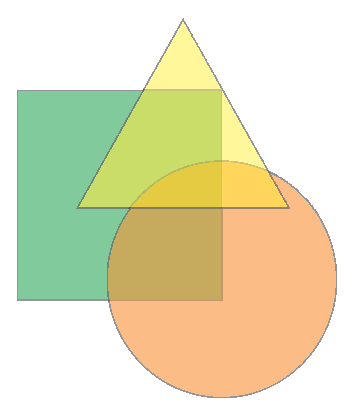
\includegraphics[width=0.7\textwidth]{Bilder/Grafik}		
		%\captionof{figure}{ Grafiken}	
			%\label{fig:GrafikOptionen}
  	\end{minipage}	
 	\hfill 	
  	\begin{minipage}[c]{0.7\textwidth}
  		\blindtext
  	\end{minipage}  
	\par\endgroup
\end{minipage}


% \begin{minipage}[t]{0.6\textwidth}
%	\begingroup
%	\parfillskip=0pt
%	% zwei weitere Minipages
%	\begin{minipage}[t]{0.47\textwidth}
%	\blindtext
%	\end{minipage}%
%	\hfill
%	\begin{minipage}[t]{0.47\textwidth}
%	\blindtext
%	\end{minipage}%
%	\par\endgroup
%\end{minipage}


%Technische Mitarbeiter und Sekretariat
%Technical staff and office
\newpage

\section*{Technische Mitarbeiter und Sekretariat}

	\begin{tabular}{p{2.1cm}p{6cm}p{2cm}p{6cm}}
	% 1. row
	\parbox[c]{2cm}{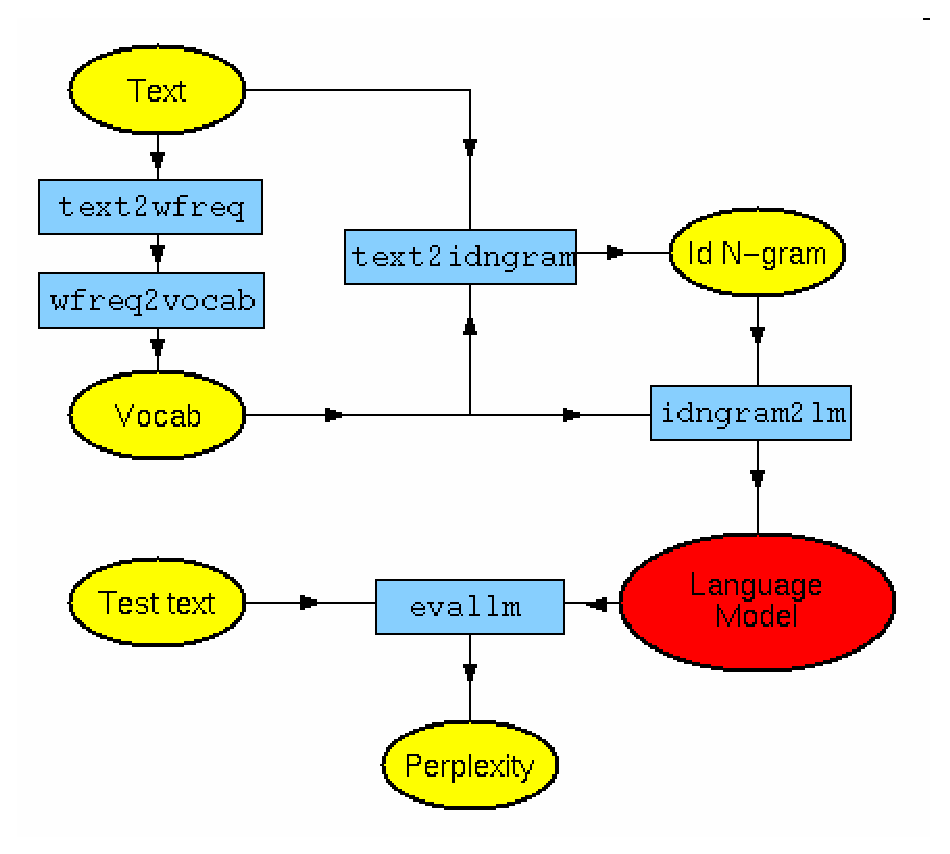
\includegraphics[width=2cm]{Bilder/toolkit.eps}} 	\hfill 	 	
	& \parbox[c]{5.9cm}{
			Dipl.Ing Wilhelm Peters\\
			Studium der Elektrotechnik\\
			\enfont{Studies in electrical engineering}\\
			Systemoptimierung Fahrantrieb\\
			\enfont{System optimisation traction drive}\\
			\phantom{test}\\
			\phantom{test}\\
		}	
	&	\parbox[c]{2cm}{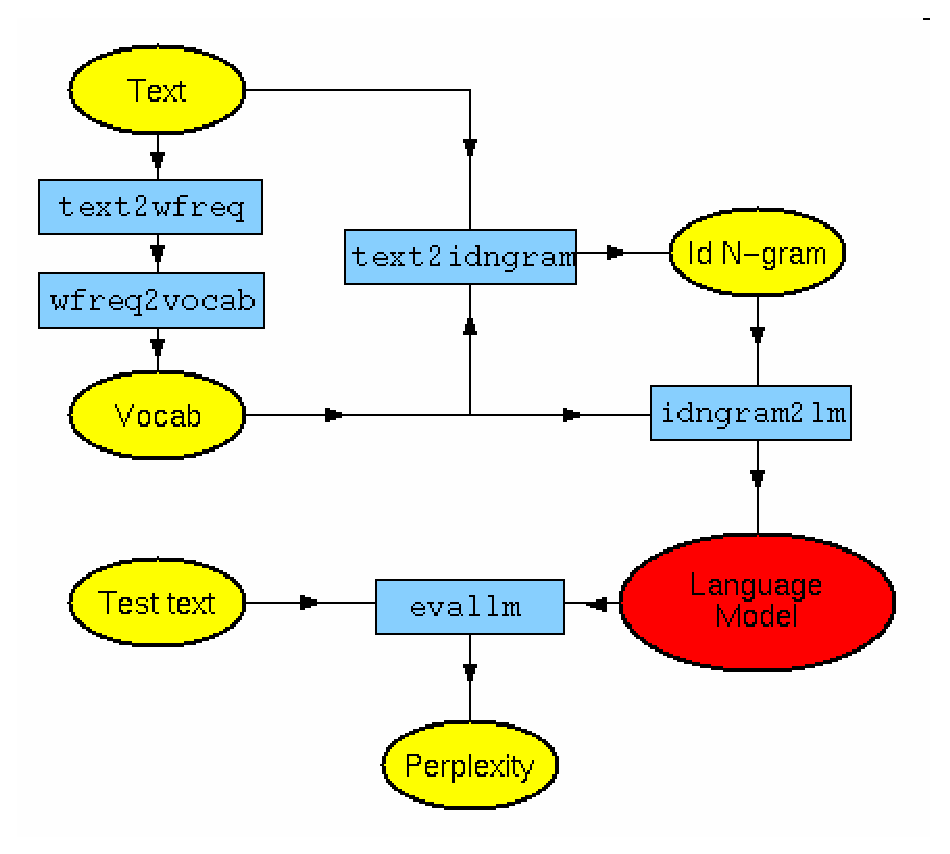
\includegraphics[width=2cm]{Bilder/toolkit.eps}}  	\hfill 		
	
	& \parbox[c]{5.9cm}{
			Dipl.Ing Wilhelm Peters\\
			Studium der Elektrotechnik\\
			\enfont{Studies in electrical engineering}\\
			Systemoptimierung Fahrantrieb\\
			\enfont{System optimisation traction drive}\\
			Mitarbeiter seit 2007
			\enfont{Member of staff since 2007}\\
		}\\
		%\phantom{Leerzeile} &&&\\
		
	% 2. row
	\parbox[c]{2cm}{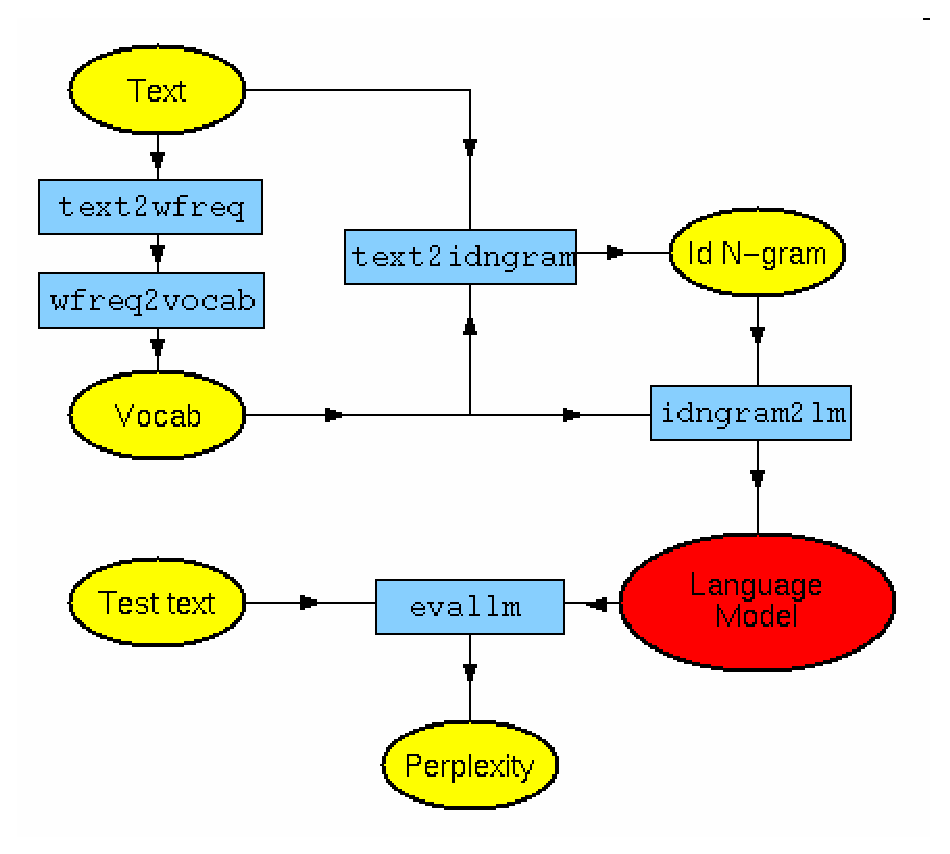
\includegraphics[width=2cm]{Bilder/toolkit.eps}} 	\hfill 	
	& \parbox[c]{5.9cm}{
			Dipl.Ing Wilhelm Peters\\
			Studium der Elektrotechnik\\
			\enfont{Studies in electrical engineering}\\
			Systemoptimierung Fahrantrieb\\
			\enfont{System optimisation traction drive}\\
			\phantom{test}\\
			\phantom{test}\\
		}	
		
	&	\parbox[c]{2cm}{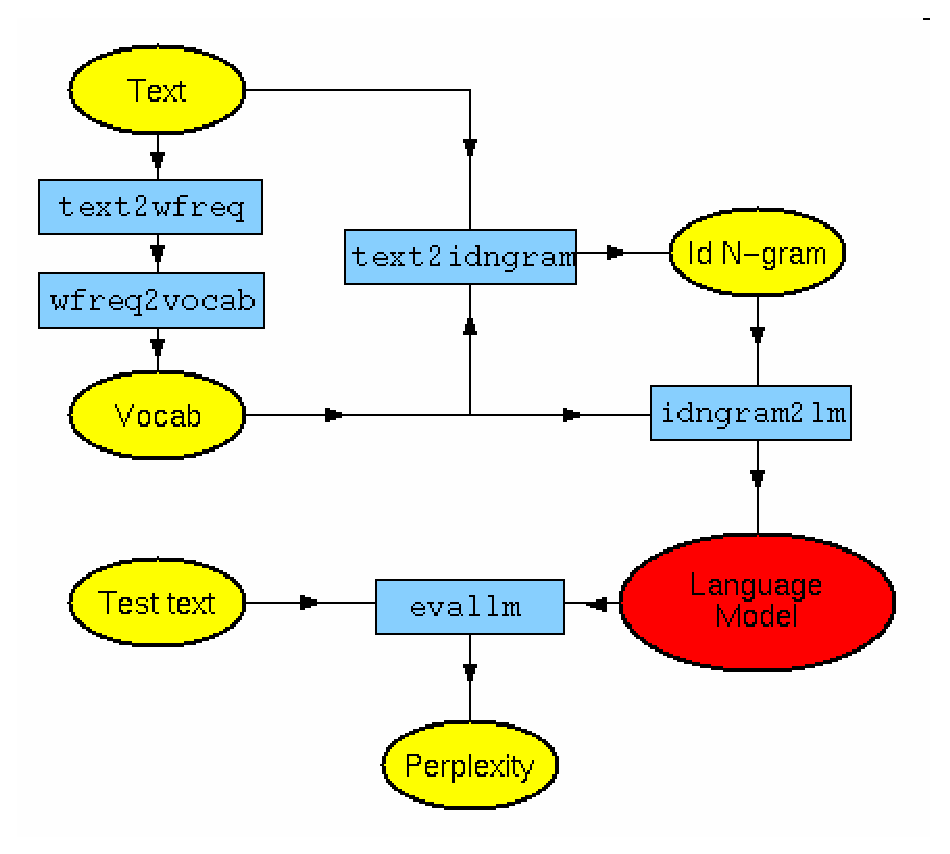
\includegraphics[width=2cm]{Bilder/toolkit.eps}}  	\hfill 	
	& \parbox[c]{5.9cm}{
			Dipl.Ing Wilhelm Peters\\
			Studium der Elektrotechnik\\
			\enfont{Studies in electrical engineering}\\
			Systemoptimierung Fahrantrieb\\
			\enfont{System optimisation traction drive}\\
			Mitarbeiter seit 2007
			\enfont{Member of staff since 2007}\\
		}\\
	%	\phantom{Leerzeile} &&&\\		
\end{tabular}
%Wissenschaftliche Mitarbeiter
%Scientific staff

\section*{Wissenschaftliche Mitarbeiter}

	\begin{tabular}{p{2.1cm}p{6cm}p{2cm}p{6cm}}
	% 1. row
	\parbox[c]{2cm}{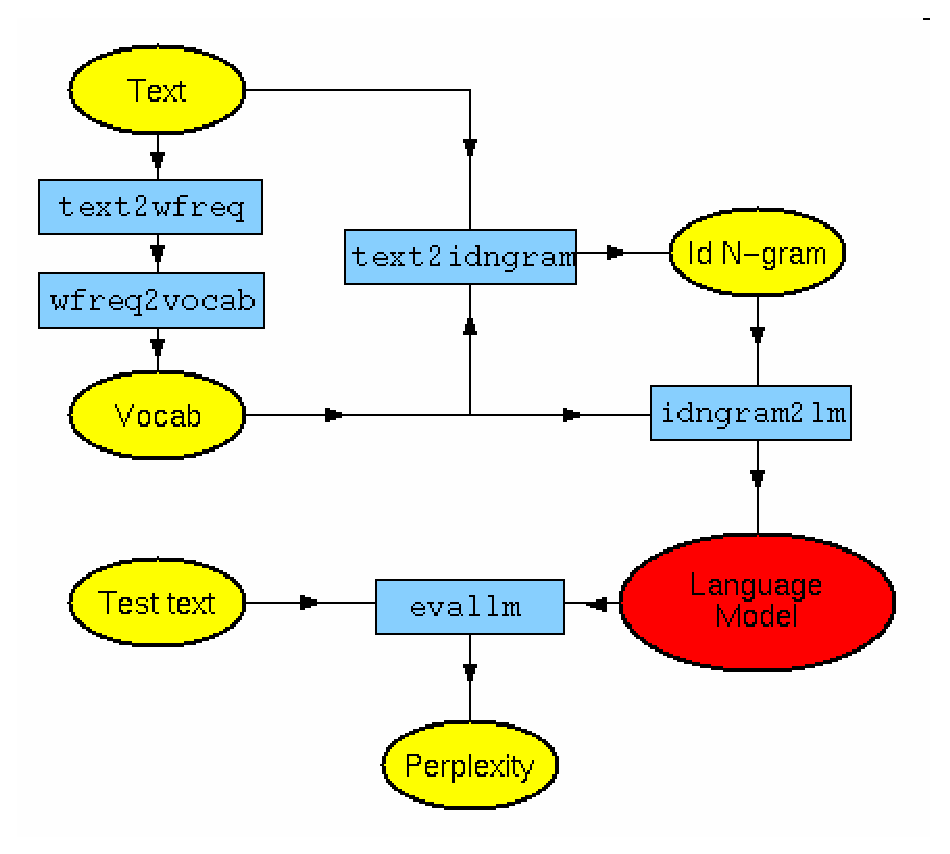
\includegraphics[width=2cm]{Bilder/toolkit.eps}} 	\hfill 	 	
	& \parbox[c]{5.9cm}{
			\Large Dipl.Ing Wilhelm Peters \normalsize \\
			\phantom{test}\\
			Studium der Elektrotechnik\\
			\enfont{Studies in electrical engineering}\\
			Systemoptimierung Fahrantrieb\\
			\enfont{System optimisation traction drive}\\
			\phantom{test}\\
			\phantom{test}\\
		}	
	&	\parbox[c]{2cm}{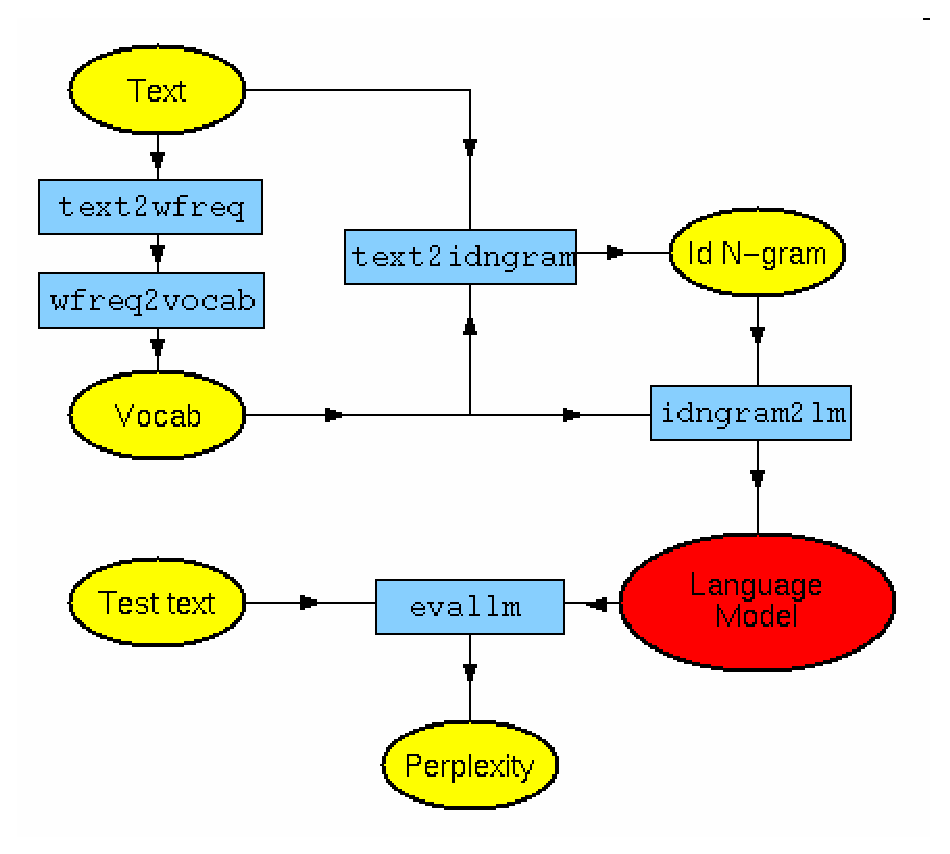
\includegraphics[width=2cm]{Bilder/toolkit.eps}}  	\hfill 		
	
	& \parbox[c]{5.9cm}{
			\Large Dipl.Ing Wilhelm Peters \normalsize \\
			\phantom{test}\\
			Studium der Elektrotechnik\\
			\enfont{Studies in electrical engineering}\\
			Systemoptimierung Fahrantrieb\\
			\enfont{System optimisation traction drive}\\
			Mitarbeiter seit 2007
			\enfont{Member of staff since 2007}\\
		}\\
		%\phantom{Leerzeile} &&&\\
		
	% 2. row
	\parbox[c]{2cm}{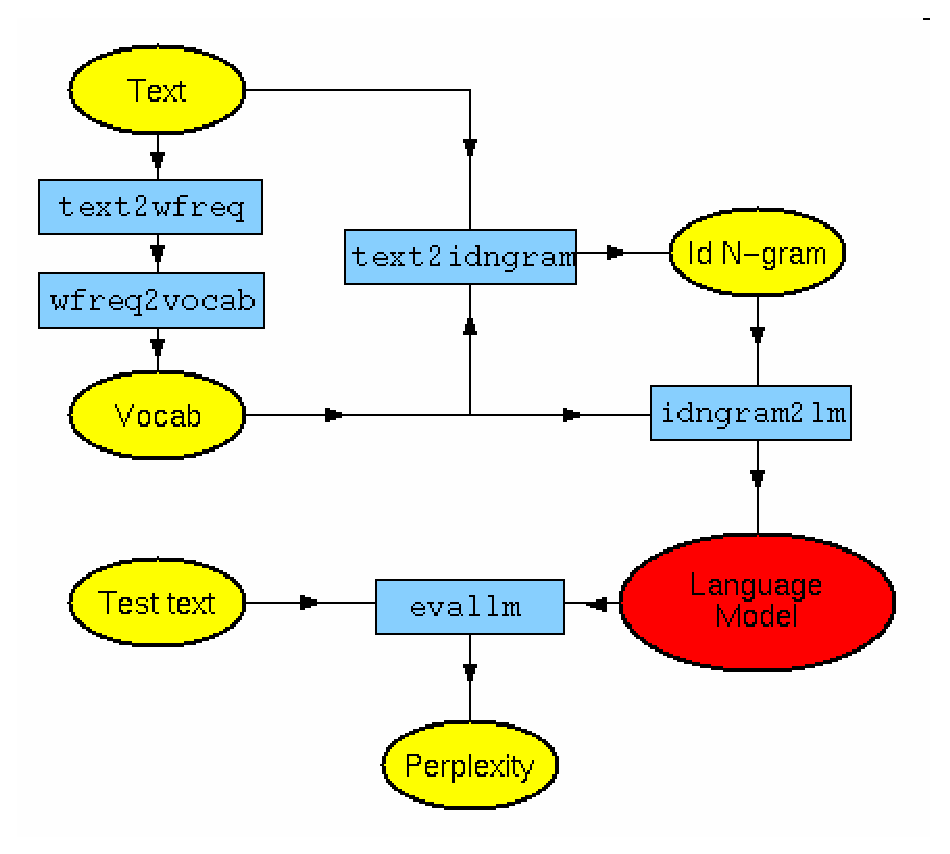
\includegraphics[width=2cm]{Bilder/toolkit.eps}} 	\hfill 	
	& \parbox[c]{5.9cm}{
			\Large Dipl.Ing Wilhelm Peters \normalsize \\
			\phantom{test}\\
			Studium der Elektrotechnik\\
			\enfont{Studies in electrical engineering}\\
			Systemoptimierung Fahrantrieb\\
			\enfont{System optimisation traction drive}\\
			\phantom{test}\\
			\phantom{test}\\
		}	
		
	&	\parbox[c]{2cm}{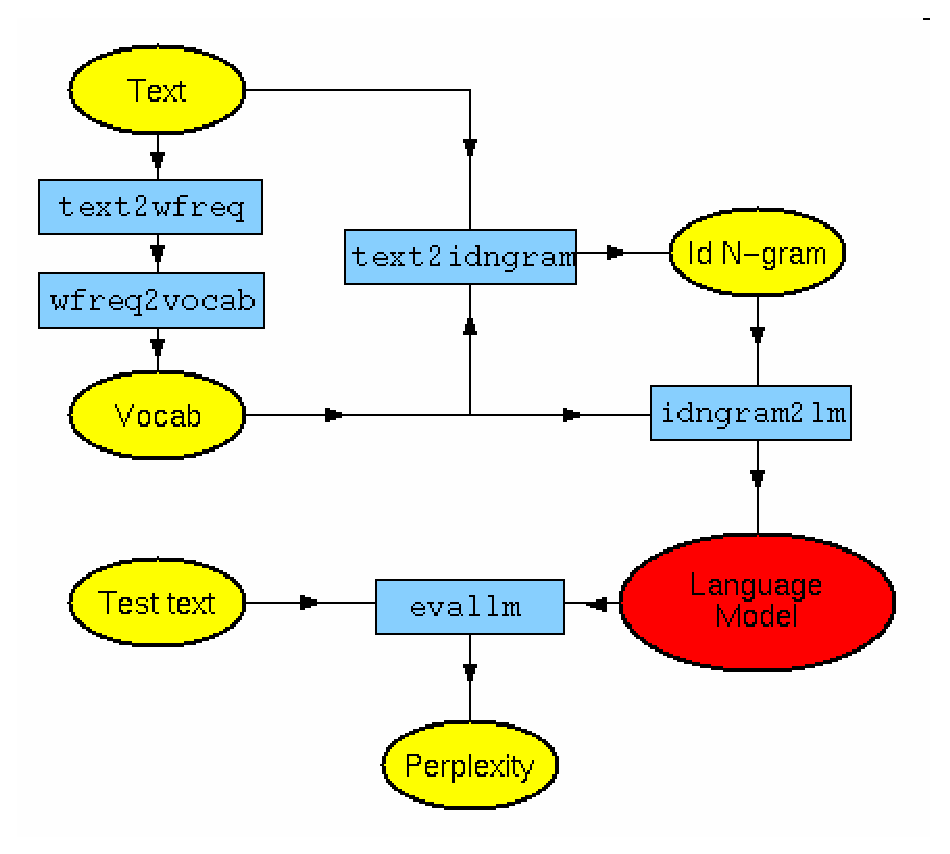
\includegraphics[width=2cm]{Bilder/toolkit.eps}}  	\hfill 	
	& \parbox[c]{5.9cm}{
			\Large Dipl.Ing Wilhelm Peters \normalsize \\
			\phantom{test}\\
			Studium der Elektrotechnik\\
			\enfont{Studies in electrical engineering}\\
			Systemoptimierung Fahrantrieb\\
			\enfont{System optimisation traction drive}\\
			Mitarbeiter seit 2007
			\enfont{Member of staff since 2007}\\
		}\\
	%	\phantom{Leerzeile} &&&\\		
\end{tabular}

Hier ist ein text. \phantom{Und hier ist der Text als phantom}. Hier ist wieder text.


\chapter{Forschungsschwepunkte}
\echapter{RESEARCH}
%\LR{
		%\subsection{sub1 Parallel} 
		%\blindtext \blindtext \blindtext \blindtext
%		}{
		%\esubsection{sub2 Parallel}
		% \blindtext \blindtext \blindtext \blindtext
%}
\input{mainmatter/forschungsschwepunkte/regelung_von_PM}

\chapter{Labor}
\echapter{Labory}


\chapter{Lehrveranstaltungen}



\chapter{Kooperationen}

%\clearpage
%\bibliographystyle{get_deu_alphadin}							% default styles  get_alphadin} %     
%\bibliographystyle{alpha}
%\bibliographystyle{get_natdin}
%\bibliographystyle{get_eng_natdin}						% f? englische Texte
%\bibliographystyle{unsrtdin}
%\bibliographystyle{bib/IEEEtran}
%\bibliography{bib/Ref_xby}

\begin{figure}
  \figbicaption{fig:test}{Deutscher Titel}{English Title}
\end{figure}



\chapter{Title of first chapter}
\begin{refsection}
This is just filler text \parencite{massa}.
This is just filler text \parencite{augustine}.
This is just filler text \parencite{cotton}.
This is just filler text \parencite{hammond}.
\printbibliography[heading=subbibliography]
\end{refsection}

\chapter{Title of second chapter}
\begin{refsection}
This is just filler text \parencite{hammond}.
This is just filler text \parencite{massa}.
This is just filler text \parencite{cotton}.
This is just filler text \parencite{murray}.
\printbibliography[heading=subbibliography]
\end{refsection}

\chapter{Title of third chapter}
\begin{refsection}
This is just filler text \parencite{murray}.
This is just filler text \parencite{augustine}.
This is just filler text \parencite{cotton}.
This is just filler text \parencite{bertram}.
\printbibliography[heading=subbibliography]
\end{refsection}  
                                     
                                        
\appendix
% Anhang
%\chapter{Anhang}
\thispagestyle{empty}
 


\addchap{Appendix}
\section{Power Distribution}
\label{app:powwer_distribution}
%Appendix_power_distribution

This section aims for offering a set of numerical functions to calculating the power distribution along beam propagation in a photonic waveguide. The simplest idea is to compute the power in waveguide and base by integrating power flow density (or Poynting vector $\vec{S}$) at their cross-sections respectively. Meanwhile CST MWS has constructed a cuboid like Fig. \ref{Afig:app_power_distribution01}, which contains all involved objects such as waveguide and TLF, as a total calculation space which is discretized through Finite Integration Technique (FIT) and all variables (see \cite{script_FeldSim} or section \ref{sect:FIT}) from FIT are also available from CST MWS. In following it will be introduced how to calculate the power distribution of a Fiber-to-Chip model (see section \ref{sect:model_simulation}). 
\begin{figure}[ht]
\centering
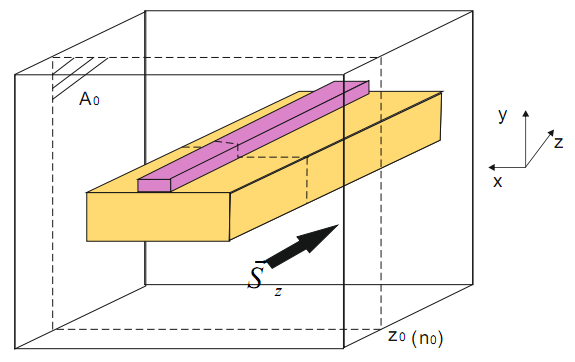
\includegraphics[width=0.7 \textwidth]{bilder/app_power_distribution01}
\caption{Calculation Cuboid in CST.}
\label{Afig:app_power_distribution01}
\end{figure}
The first step is to choose a working plane. Suppose a working plane through point z$_{0}$ at z axis in the total calculation space Fig. \ref{Afig:app_power_distribution01} is given, the point index n$_{0}$ can be determined by its coordinate z$_{0}$. The plane in Fig. \ref{Afig:app_power_distribution02} is divided into small elemental pieces in FIT. The base cross-section is given by four points coordinates (x$_{1}$, y$_{1}$),(x$_{2}$, y$_{2}$),(x$_{3}$, y$_{3}$) and (x$_{4}$, y$_{4}$). Their points indexes (n$_{1}$, n$_{2}$, n$_{3}$, n$_{4}$) can also be derived.    
\begin{figure}[ht]
\centering
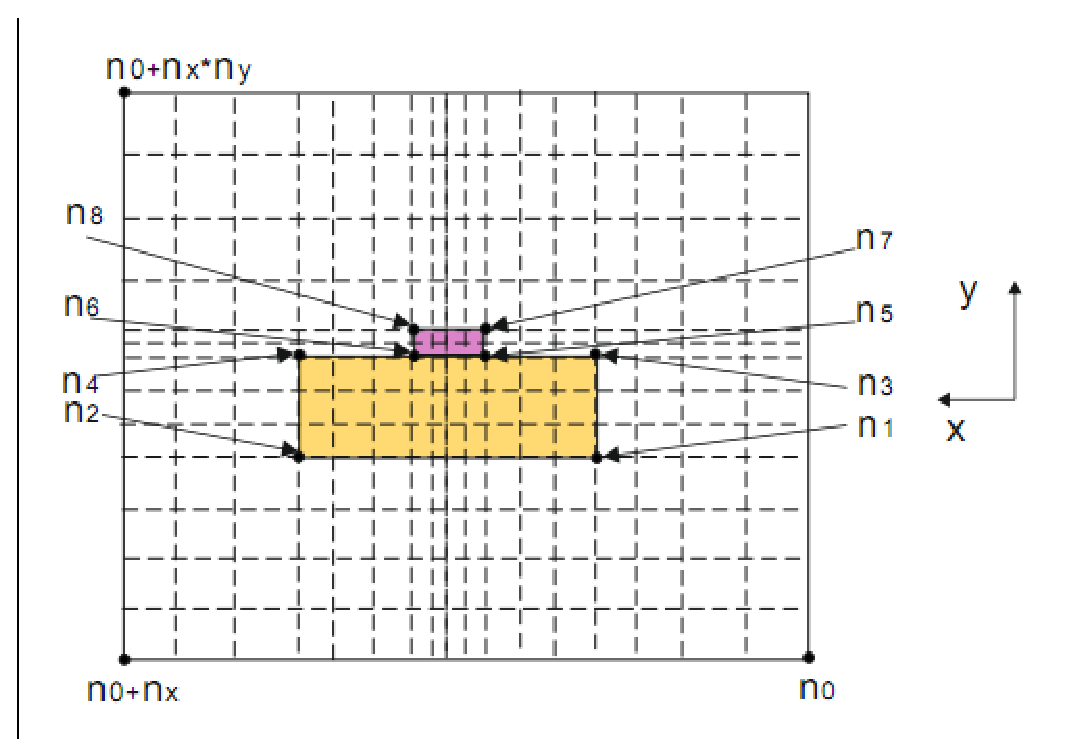
\includegraphics[width=0.7 \textwidth]{bilder/app_power_distribution02}
\caption{Cross-section at z$_{0}$.}
\label{Afig:app_power_distribution02}
\end{figure}
In the next step it is necessary to prepare variables such as elemental 
As is in \cite{script_FeldSim} the complete elemental plane matrix D$_{A}$ is given by (\ref{Aeq:da_matrix}): 
\begin{equation}
D_{A}=Diag\left\{Ax(1),\cdots,Ax(Np),Ay(1),\cdots,Ay(Np), Az(1),\cdots,Az(Np)\right\}
\label{Aeq:da_matrix}
\end{equation}

In the working cross-section only z-components of elemental plane matrix D$_{A}$ are needed:
\begin{equation}
D_{Az}=D_{A}(2*Np+1:3*Np, 2*Np+1:3*Np)
\label{Aeq:daz_matrix}
\end{equation}
Construct a auxiliary matrix $A_{base}$, which composed of only $1$ and $0$ like Fig \ref{Afig:app_Auxiliary_matrix}, to indicate all points indexes which are included in base cross-section. 

\begin{equation}
A_{base}=Diag\left\{0,\cdots 0,P_{1},0,\cdots 0, P_{2}, 0,\cdots, P_{m}, 0\cdots\right\}
\label{Aeq:A_matrix}
\end{equation}

\begin{figure}[!ht]
\centering
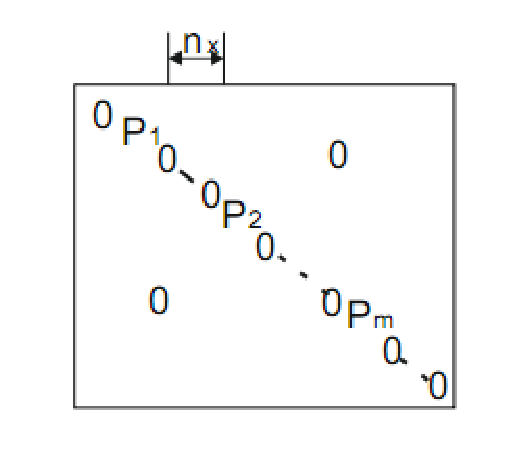
\includegraphics[width=0.5\textwidth]{bilder/app_Auxiliary_matrix}
\caption{Structure of the auxiliary matrix $A$.}
\label{Afig:app_Auxiliary_matrix}
\end{figure}
Where P$_{x}$ are submateix:
\begin{equation}
P_{x}=Diag\left\{1,\cdot,1\right\}_{(n_{2}-n_{1})*(n_{2}-n_{1})}
\end{equation}
And m is given by:
\begin{equation}
m=(n_{3}-n_{1})/n_{x}=(n_{4}-n_{2})/n_{x}
\end{equation}
Then 
\begin{equation}
D_{Abase}=A_{guide}*D_{A}
\end{equation}
Pick z-components of the Poynting vector $S$:
\begin{equation}
S_{z}=S(2*Np+1:3*Np)
\end{equation}
At last the power in base at the plane (for z=z$_{0}$) can be counted up by:
\begin{equation}
P_{base}(z)=sum(D_{Abase}*S_{z})
\end{equation}

By analogous procedures power in guide cross-section $P_{guide}$ and in total cross-section $P_{total}$ are derived. For observing the power distribution the results are processed by normalization:
\begin{align}
\eta_{guide}&=\frac{P_{guide}}{P_{total}}\\
\eta_{base}&=\frac{P_{base}}{P_{total}}\\
\eta_{air}&=1-\eta_{guide}-\eta_{base}
\end{align}



\section{Spot Size Curve}
\label{app:spot_size}
%Appendix_spot_size
In this section we will introduce the process of calculating beam spot size from data in CST MWS. As definition of spot size, the target is the distance from beam center to the point where the power density is $1/e^{2}$ of the peak value.  Fig. \ref{Afig:beam_cuboid} is the calculation cuboid in the CST MWS. The gaussian beam propagates along the z-axis in the simulation of this work. So the spot diameter is the function of z coordinate $d=f(z)$. In order to calculate the spot diameter we cut a working plane at each z-coordinate. Like the step in Appendix \ref{app:powwer_distribution}, we assume a working plane through the point $z_{0}$. In this work the simulation of beam propagation is symmetric on both x-axis and y-axis. Thus only quarter of the beam cross-section is the working plane like Fig. \ref{Afig:beam_crosssection} in CST MWS. Supposing the point $n_{0}$ is the beam center of this plane the peak value of the power flow density is $|S(n_{0})|$. The next step is to find the point $n_{1}$ where $|S(n_{1})|=1/e^{2}|S(n_{0})|$. $n_{1}$ is also among the range $[n_{0}, n_{0}+n_{x}n_{y}]$. Point $n_{1}$ leads to its coordinate ($x_{1},y_{1}$). Then the beam spot radium of this plane is given by \ref{eq:spot_radium}. The spot size is twice of this radium. We can draw the spot size curve by joining values of the spot size in each corss-section.
\begin{figure}[!ht]
\centering
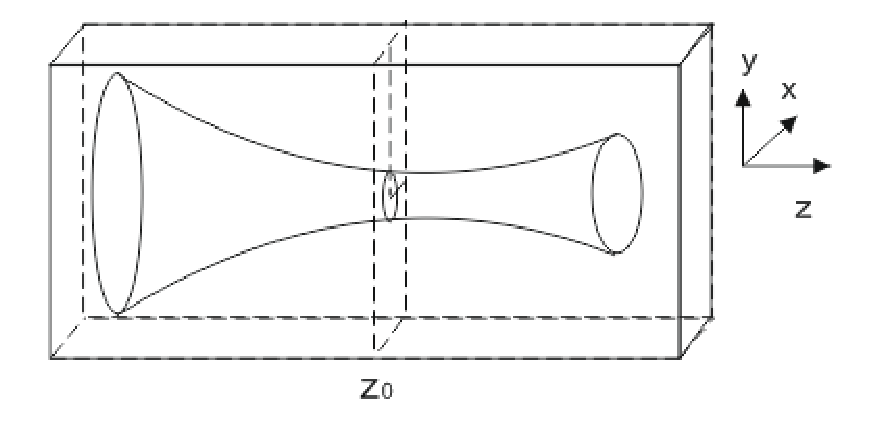
\includegraphics[width=0.5\textwidth]{bilder/beam_cuboid}
\caption{Beam propagation in simulation cuboid.}
\label{Afig:beam_cuboid}
\end{figure}
\begin{figure}[!ht]
\centering
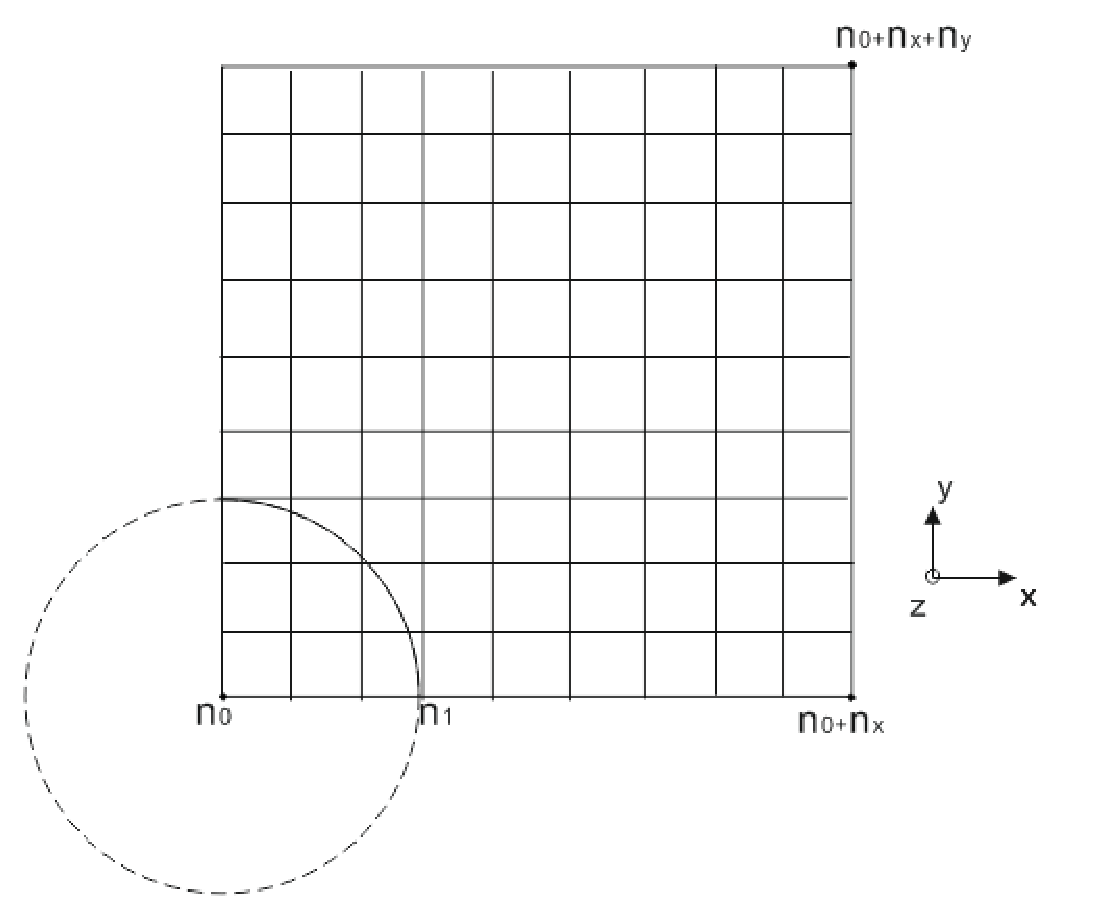
\includegraphics[width=0.5\textwidth]{bilder/beam_crosssection}
\caption{Beam cross-section at through point $n_{0}$.}
\label{Afig:beam_crosssection}
\end{figure}
\begin{equation}
R=sqrt(x_{1}^{2}+y_{1}^{2})
\label{eq:spot_radium}
\end{equation}


                                         % Schluss
%Literaturverzeichnis
% Glossar
\addchap{Symbolverzeichnis}
\thispagestyle{empty}
\label{cha:Symbole} 



\begin{longtable}{ll}

Symbolname&Bedeutung\\

\end{longtable}



% Abk�rzungsverzeichnis
%%\addchap{Abk�rzungsverzeichnis}
\addchap{Abbreviation}
\thispagestyle{empty}
\label{cha:abkurz} 
\textbf{FIT}\quad Finite Integration Theory\\
\textbf{SMF}\quad Single Mode Fiber\\
\textbf{SPP}\quad Surface Plasmon Polariton\\
\textbf{TLF} \quad Tapered Lensed Fqiber\\


\begin{spacing}{1.0}                    % Verzeichnisse werden mit einzeiligem Abstand gesetzt
%\bibliographystyle{get_deu_alphadin}							% default styles  get_alphadin} %     
%\bibliographystyle{alpha}
%\bibliographystyle{get_natdin}
%\bibliographystyle{get_eng_natdin}						% f�r englische Texte
\bibliographystyle{unsrtdin}
\bibliography{backmatter/Bibliography}						% Datei 'literatur.bib' wird eingebunden  
\nocite{*}											% include alle Eintr�ge              % Literaturverzeichnis

\end{spacing}
%Anh�nge

%% Index
Falls gew�nscht kann hier ein Index erstellt werden. (optional)

Dazu m�ssen im Text alle W�rter, die im Index auftauchen sollen mit dem Befehl 
\begin{verbatim}
\index{Befehl}
\end{verbatim}
f�r den Index markiert werden.

Der Index wird dann mit
\begin{verbatim}
\printindex
\end{verbatim}
erstellt werden.

Weitere Informationen bez�glich Indexerstellung sind in der beigef�gten Datei "`/dokumente/makeidx.pdf"' enthalten.

Das fertige Indexverzeichnis sieht dann so aus: (siehe Folgeseite)
\printindex






%%\printnomenclature[2cm]
%\cleardoubleemptypage
%\listoftables                           % Tabellenverzeichnis
%(optional)
\listoffigures                          % Abbildungsverzeichnis
%(optional)

% Die Eidesstattliche Erklaerung auf einer rechten Seite beginnen
\addchap{Erkl�rung}
\thispagestyle{empty}

\vspace*{4cm}

Hiermit versichere ich, dass ich die vorgelegte Diplomarbeit selbst�ndig angefertigt und keine anderen als die angegebenen Quellen und Hilfsmittel verwendet habe.

\bigskip
\bigskip 
\bigskip 
\bigskip 
\bigskip 

\begin{flushright}
\begin{tabular}{c}
%Paderborn, den dd. month yyyy\\
Paderborn, \today\\%dd. month yyyy\\
\bigskip \\
\hrulefill \\
%\dotfill \\
Buyu Xiao\\
\hspace{5cm} \\
\end{tabular}
\end{flushright}
               % Eidesstattliche Erklaerung

\end{document}
